\chapter{High throughput infrastructure for system genetics}
\thispagestyle{empty}
\label{chap:xqtlwormbench}

\emph{The major challenge in bioinformatics comes from the huge amount of data collected and the 
multitude of technologies used. We developed the xQTL workbench system\cite{Arends:2012} to store 
large amounts of phenotype and genotype data in the XGAP \cite{Swertz:2010a} dataformat. An 
application of the xQTL system is found in the WormQTL database \cite{Snoek:2012}.}

\null
\vfill

\begin{myexampleblock}{Originally published as:}
  \authors{Morris A Swertz, Martijn Dijkstra, ..., Danny Arends, George Byelas, et al}\\
  \emph{The MOLGENIS toolkit: rapid prototyping of biosoftware at the push of a button}\\
  \bold{BMC Bioinformatics} (2010)\\\\

  \authors{Morris A Swertz, K Joeri v/d Velde, Bruno M Tesson, ..., Danny Arends, et al}\\
  \emph{XGAP: a uniform and extensible data model and software platform for genotype and phenotype experiments}\\
  \bold{Genome Biology} (2010)\\\\

  \authors{Danny Arends*, K. Joeri v/d Velde*, Pjotr Prins, Karl W. Broman, et al.}\\
  \emph{xQTL workbench: a scalable web environment for multi-level QTL analysis}\\
  \bold{Bioinformatics} (2012)\\\\

  \authors{Danny Arends*, L. Basten Snoek*, Joeri v/d Velde*, Yang Li*, et al.}\\
  \emph{WormQTL: Public archive and analysis web portal for natural variation data in Caenorhabditis spp}\\
  \bold{Nucleic Acids Research} (2012)
\end{myexampleblock}

\newpage

\begin{wrapfigure}{r}{0.5\textwidth}
  \centering
  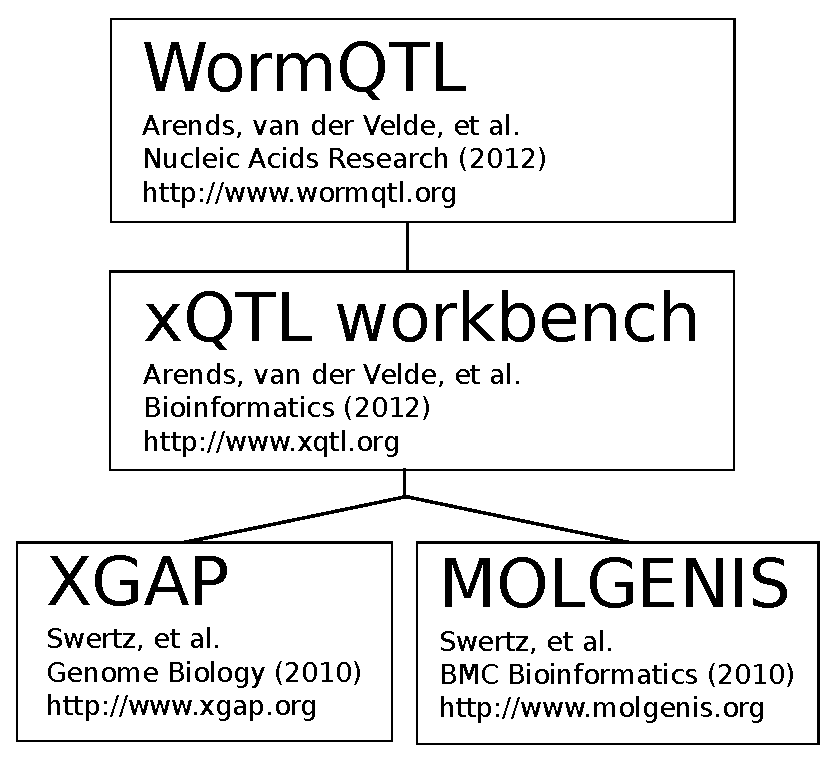
\includegraphics[width=0.4\textwidth]{eps/image_5_0.eps}
  \caption[Overview]
    {Overview of this chapter and how the different parts of this chapter are related to eachother.}
    \label{fig:Overview}
\end{wrapfigure}

This chapter deals with the storage of big data and the need to perform complex analysis in reasonable time on them.
Imagine a factory, our foundation is MOLGENIS a generator to create 'Create Read Update Delete' (CRUD) database 
applications on top of several different data storages. XGAP can be seen as the  walls of the factory, the datamodel 
defines what space is given to each object stored and how it is archived. The combined xQTL workbench system can be 
seen as the plumbing and electrics making it possible to work with the different kinds of data stored in the factory. 
The vanilla xQTL workbench comes with several tools for QTL mapping and provides ways for users to add new tools to 
the system. This chapter end by showing a real life database system actively used in \emph{C. elegans} research (Figure \ref{fig:Overview}).

\section{Reusable software (MOLGENIS)}
\subsection{Background}
High throughput technologies have boosted biological and medical research and the need for software 
infrastructures to manage and process the large datasets produced is widely accepted \cite{Swertz:2007,
Stein:2008, Thorisson:2009}. Bioinformaticians are under continuous pressure to both tackle the complexity 
and diversity of new biological systems and analytical methods and to translate these quickly into 
flexible informatics infrastructures, while keeping up with the unpredictable evolution of molecular 
biotechnologies and the increasing scale of experiments. While standardization of tools and data formats 
in open source projects like the Generic Model Organism Database, GMOD \cite{OConnor:2008}, and the 
Open Bioinformatics Foundation, OBF \cite{OBF:2010:Online}, have been indispensable in reducing the 
development efforts needed via reusable and easy to integrate components, new research must also be 
quickly accommodated, for which efficient software variation mechanisms are needed.

We present the evolution of MOLGENIS into a generic, model-driven toolkit for the rapid generation of 
data-intensive biosoftware applications \cite{Swertz:2010a}. Figure \ref{fig:modelDrivenDevelopment} 
outlines the 'model-driven' development method that several bioinformatics projects adopted in recent 
years to enable fast and flexible infrastructure development. We demonstrate step-by-
step how bioinformaticians can use a domain-specific language to efficiently model the biological 
details of their particular biological system, and use MOLGENIS software generation tools to 
automatically generate a web application tailored to the experiments of their biologists, 
building on reusable components. Next, we evaluate the results of these methods in the development 
of a range of MOLGENIS applications \cite{Swertz:2004, Swertz:2010a, Thorisson:2009, Leu:2010, 
Li:2009, Smedley:2008}, that is, software applications generated using the MOLGENIS toolkit. We found 
up to 30 times efficiency improvement compared to hand-writing software, while providing a richness 
of features practically unfeasible to produce by hand but not yet provided by related projects. We 
conclude by inviting the bioinformatics community to add more MOLGENIS models, components and 
generators to quickly generate all the software infrastructures biologists want to have.

\begin{figure}[ht!]
  \centering
  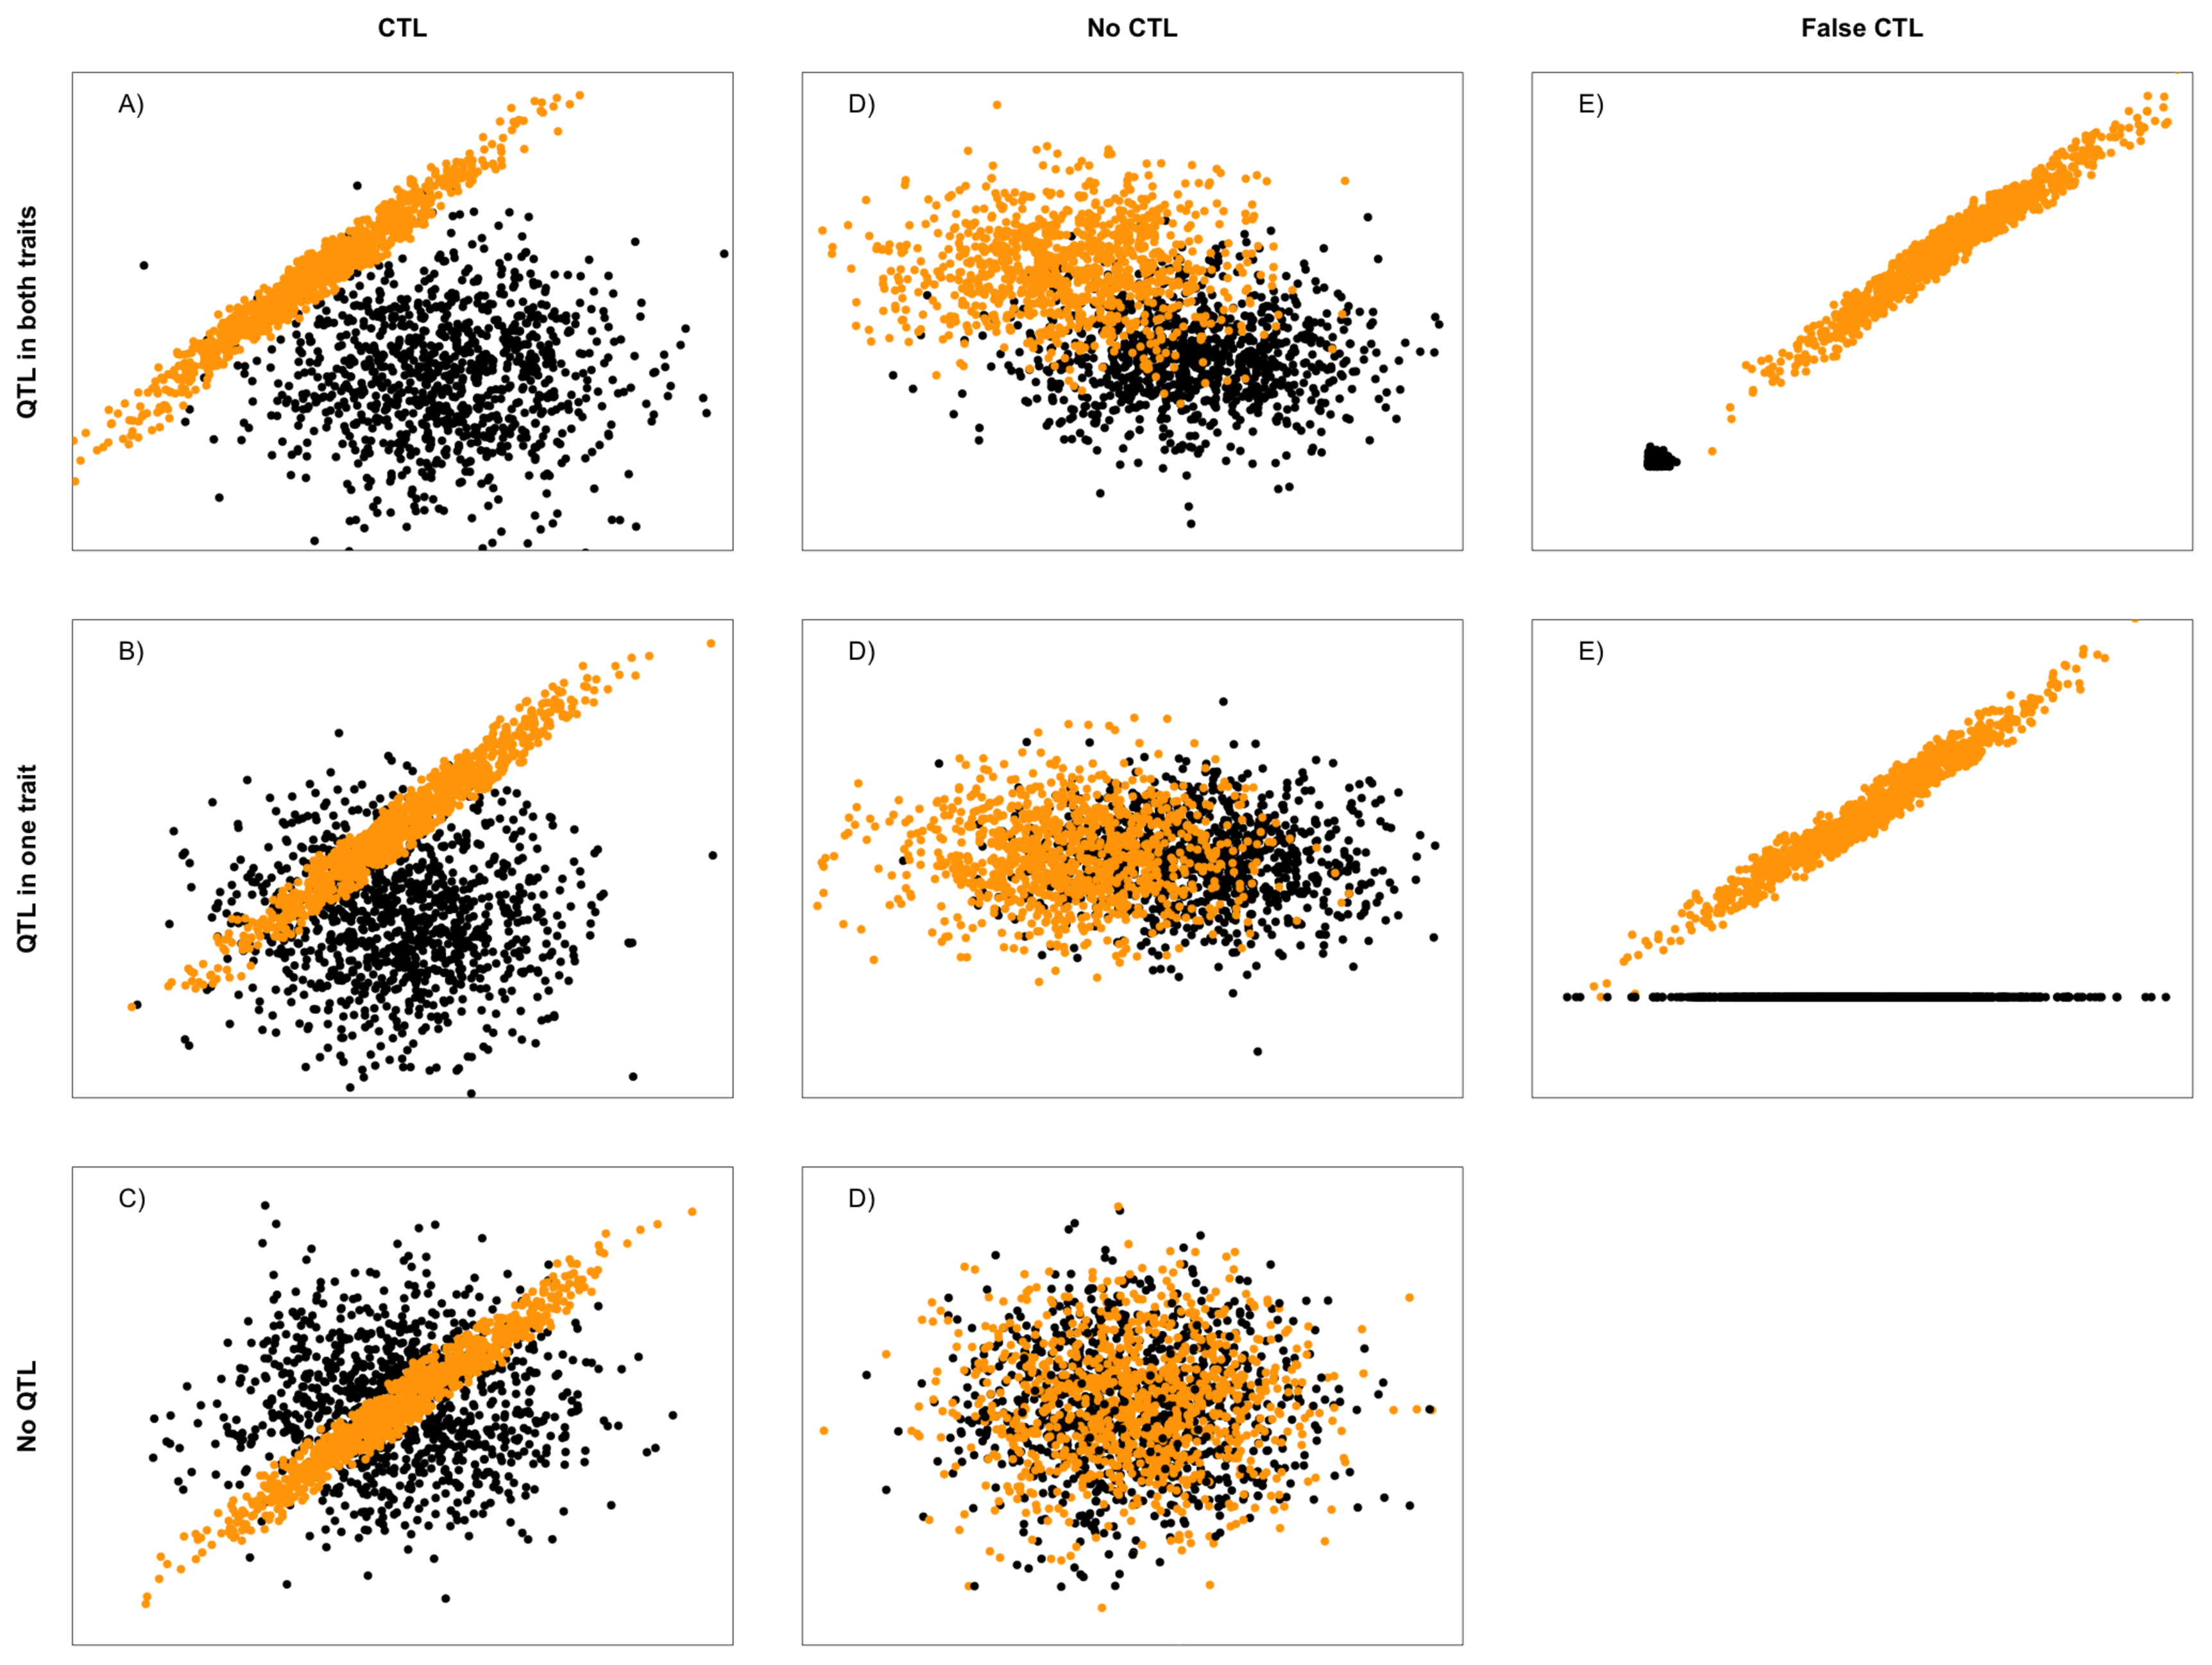
\includegraphics[width=1.0\textwidth]{eps/image_5_1.eps}
  \caption[MOLGENIS]
    {Many minor and major changes have to be written in software code before a 'standard' software infrastructure 
    accommodates a particular research. Using 'model-driven' development methods a bioinformatician only need to 
    model what is needed for his experiment using a therefore optimized domain specific language (DSL). Generators 
    quickly produce all the software logic to compose a full software infrastructure that accommodates these needs. 
    When experimental needs change, a bioinformatician can (re)run the same generator with an adapted model file 
    to quickly produce another variant of software infrastructure. This vastly reduces 'time-to-research' and 
    enables bioinformaticians to quickly develop a suite of software infrastructures, with each variant accommodating 
    a specific research task, while still on track to reuse, integrate and share the best standard features with 
    other labs and bioinformaticians.}
    \label{fig:modelDrivenDevelopment}
\end{figure}

The MOLGENIS toolkit is based on the method of model-driven development which emerged in the 1990s 
from the computer industry. Below we discuss the MOLGENIS' modeling language, the generators and 
reusable components. 

\subsubsection{Modeling language}
A custom MOLGENIS application can be defined in a single file. The file is written in MOLGENIS' 
modeling language. One can think of MOLGENIS' modeling language as a 'domain-specific language' 
\cite{Deursen:2002}, in this case to compose biosoftware infrastructures.

In most cases, knowledge of the DSL is all that is needed to produce a custom MOLGENIS application 
variant. The domain-specific language was implemented using XML so that model files can be edited 
using off-the-shelf XML editors. However, you may want to include hand-programmed components into 
a particular MOLGENIS instance. For example, for the eXtensible Genotype And Phenotype (XGAP) 
database application of MOLGENIS \cite{Swertz:2010a}, we developed a 'MatrixViewer' that builds on the generated 
components, which saved us the work of writing the plug-in from scratch. This requires a model 
sentence that points to the 'plug-in' (allowing it to be seamlessly integrated) as well as 
hand-programming of the plug-in itself.

\subsubsection{Reusable components}
Each MOLGENIS application follows the widely accepted three-layered architecture design of web 
applications. MOLGENIS' reusable components provide building blocks with a modular structure, which 
allows them to be assembled in diverse combinations, similar to prefabricated houses that are built 
from modular walls instead of bricks. Some building blocks are semi-finished and need to be 
'completed' before use (which is automated in MOLGENIS via the generators and inheritance). We based 
the design of MOLGENIS on industry-proven design patterns from the 'patterns for enterprise 
application architecture' (PEAA), a catalog of proven solutions for software design problems 
that we used as a guideline \cite{Fowler:2002}. The logic of the reusable components is implemented using 
Java (\url{http://java.sun.com/}); the HTML layout for the user interface is encoded in Freemarker 
templates (\url{http://freemarker.sourceforge.net/}); and the database back-end using MySQL, PostgreSQL 
or HSQLDB.

\begin{figure}[h!]
  \centering
  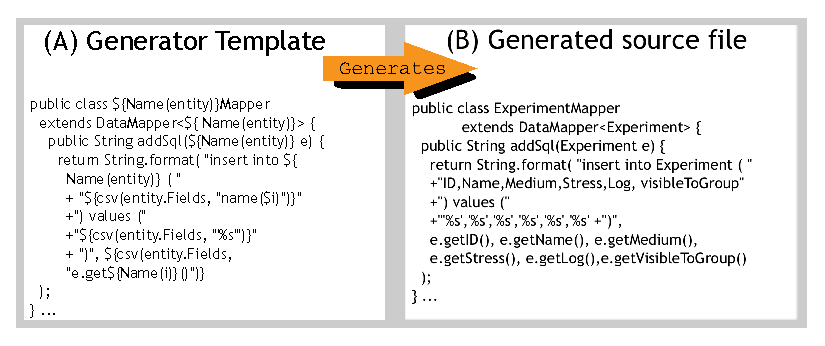
\includegraphics[width=1.0\textwidth]{eps/image_5_2.eps}
  \caption[Templates]
    {MOLGENIS generators are implemented as templates. This example shows the generator for a database component 
    (A). This template is applied to each <entity> in the model to generate many complete DataMappers that would 
    otherwise need to be written by hand. (B) shows an example of the generated source files, in this case for 
    <entity name="Experiment"> as described in Figure 1. The command \$Name(entity) translates to the name of the 
    entity ("Experiment") and command \${csv(\$entity.Fields, x)} means that command 'x' is applied to each field 
    of the entity and returned as a comma separated string (csv).}
	\label{fig:Generators}
\end{figure}

\subsubsection{Generators}
The generators are compact specifications of how each database feature should be implemented. 
The MOLGENIS toolkit now has over 20 generators, but normal users will never need to take a look 
inside. However, for readers wanting to create their own generators, figure \ref{fig:Generators} provides an example 
of the simple, text-based, generators we use. Each generator consists of two files: a Freemarker 
template that describes the code to be generated (similar to that shown in figure \ref{fig:Generators}a) and a Java 
'Generator' class that controls the generating process. A new generator can be developed as 
follows: First write some examples of the desired programs by hand, where possible using similar 
patterns and mark which parts are variable between them. Then copy one of these examples into 
a generator template (text file) and replace all variable parts with 'holes' that 
are to be filled by the code generator based on parameters from DSL. At each generation, the 
template is then automatically copied and the 'holes' filled, based on parameters described in 
the domain-specific language, saving much laborious manual work. 

\subsection{Results}
To start generating your own MOLGENIS application, you can download a ready-to-use 'workspace' 
from \url{http://www.molgenis.org/}, which can be edited using the commonly used Eclipse integrated 
development environment (IDE) tool (\url{http://www.eclipse.org/}). Extensive manuals are available to 
help install the Java, MySQL, Tomcat and Eclipse software needed and to learn how to walk through 
the Eclipse workspace to edit models and generate and run MOLGENIS instances; most new users can 
complete this part in about three hours. Below we summarize the output you can expect as well 
as recent experiences from using this toolbox. Detailed examples on how these features can be 
used to support actual microarray or genetical genomics experiments can be found in \cite{Swertz:2010a, Li:2009, Smedley:2008}.

After completing a MOLGENIS model and running the generator as described above, you have a 
ready-to-use software application. The features you get when running the generated result as 
a web application: a fully functional system where researchers can upload, manage, browse 
and query their biological data that conform to the model, optionally enhanced with analysis 
tools to explore and annotate (depending on the plug-ins).

\subsubsection{Applications}
Since the earliest MOLGENIS application \cite{Swertz:2004}, we have successfully evaluated use of 
the MOLGENIS toolkit to build a wide range of biomedical applications \cite{Swertz:2010a, Fredman:2002, 
Leu:2010, Li:2009, Smedley:2008}, ranging from sequencing to proteomics.A full list MOLGENIS applications 
can be found at \url{http://www.molgenis.org/}. Each of these MOLGENIS projects reported major benefits 
from the short cycle from model to running system to enable quick evaluation (500 lines of model XML 
replaces 15,000 lines of programming code) and use of the batch loading of data to evaluate how the newly 
built system works with real data. More often than not, MOLGENIS helped in finding inconsistencies in 
existing data that would otherwise have gone unnoticed, leading to experimental errors. In our experience, 
a typical MOLGENIS generator run gives you about 90\% of the application that is desired 'for free', with the 
remaining 10\% typically filled in using plug-ins that are written by hand. The MOLGENIS toolkit has also 
been used to extend or replace existing software applications: the ExtractModel tool allows you to generate 
a MOLGENIS application from an existing database, which can then be run side-by-side with code developed 
previously, providing the best of both generated and hand-written worlds.

\subsection{Conclusions and Discussions}
In a recent perspective paper \cite{Swertz:2007} we evaluated the general benefits and pitfalls of model-driven 
development, such as the ability to develop infrastructure in short cycles to get the application 
right, ensuring developers and biologists are thinking along the same lines and increasing quality 
and functionality for all. We further evaluated applying this method to both microarray and genetical 
genomics experiments \cite{Swertz:2004}, \cite{Swertz:2010a}.

We conclude that using model-driven methods enables bioinformaticians to build biological software 
infrastructures faster than before, with the additional benefit of much easier sharing of models, data 
and components. Much less time is spent on customizing and gluing together individual components. The 
result is of higher quality because fewer incidental errors creep into the applications as a consequence 
of the automated procedures; best practices are applied instead of reinvented. And you do not need 
heavy-weight technology to implement a model-driven generator: simple text-based templates suffice to 
create biological software generators.

\section{Storing extensible data (XGAP)}
We present an extensible software model for the genotype and phenotype community, XGAP. Readers 
can download XGAP (\url{http://www.xgap.org/}) or auto-generate a custom version using 
MOLGENIS with programming interfaces to R-software and web-services or user interfaces for 
biologists. XGAP has simple load formats for any type of genotype, epigenotype, transcript, 
protein, metabolite or other phenotype data. Current functionality includes tools ranging 
from eQTL analysis in mouse to genome-wide association studies in humans.

\subsection{XGAP - A minimal and extensible object model}
We developed the XGAP objectmodel to uniformly capture the wide variety of (future) genotype 
and phenotype data, building on generic standard model FuGE (Functional Genomics Experiment) 
\cite{Jones:2007} for describing the experimental 'metadata' on samples, protocols and experimental variables 
of functional genomics experiments, the OBO model (of the Open Biological and Biomedical 
Ontologies foundry for use of standard and controlled vocabularies and ontologies that ease 
integration \cite{Smith:2007}, and lessons learned from previous, profiling 
technology-specific modeling efforts \cite{Brazma:2006}.

Figure \ref{fig:XGAP}b shows the core components of a genotype-to-phenotype investigation: the biological 
subjects studied (for example, human individuals, mouse strains, plant tissue samples), the 
bio molecular protocols used (for example, Affymetrix, Illumina, Qiagen, liquid 
chromatography/mass spectrometry (LC/MS), Orbitrap, NMR), the trait data generated (usually 
data matrices with, for example, phenotype or transcript abundance data), the additional 
information on these traits (for example, genome location of a transcript, masses of LC/MS peaks), 
the wet-lab or computational protocols used (for example, MetaNetwork \cite{Fu:2007} in the case of QTL and
network analysis) and the derived data (for example, QTL likelihood curves).

\begin{figure}[ht!]
  \centering
  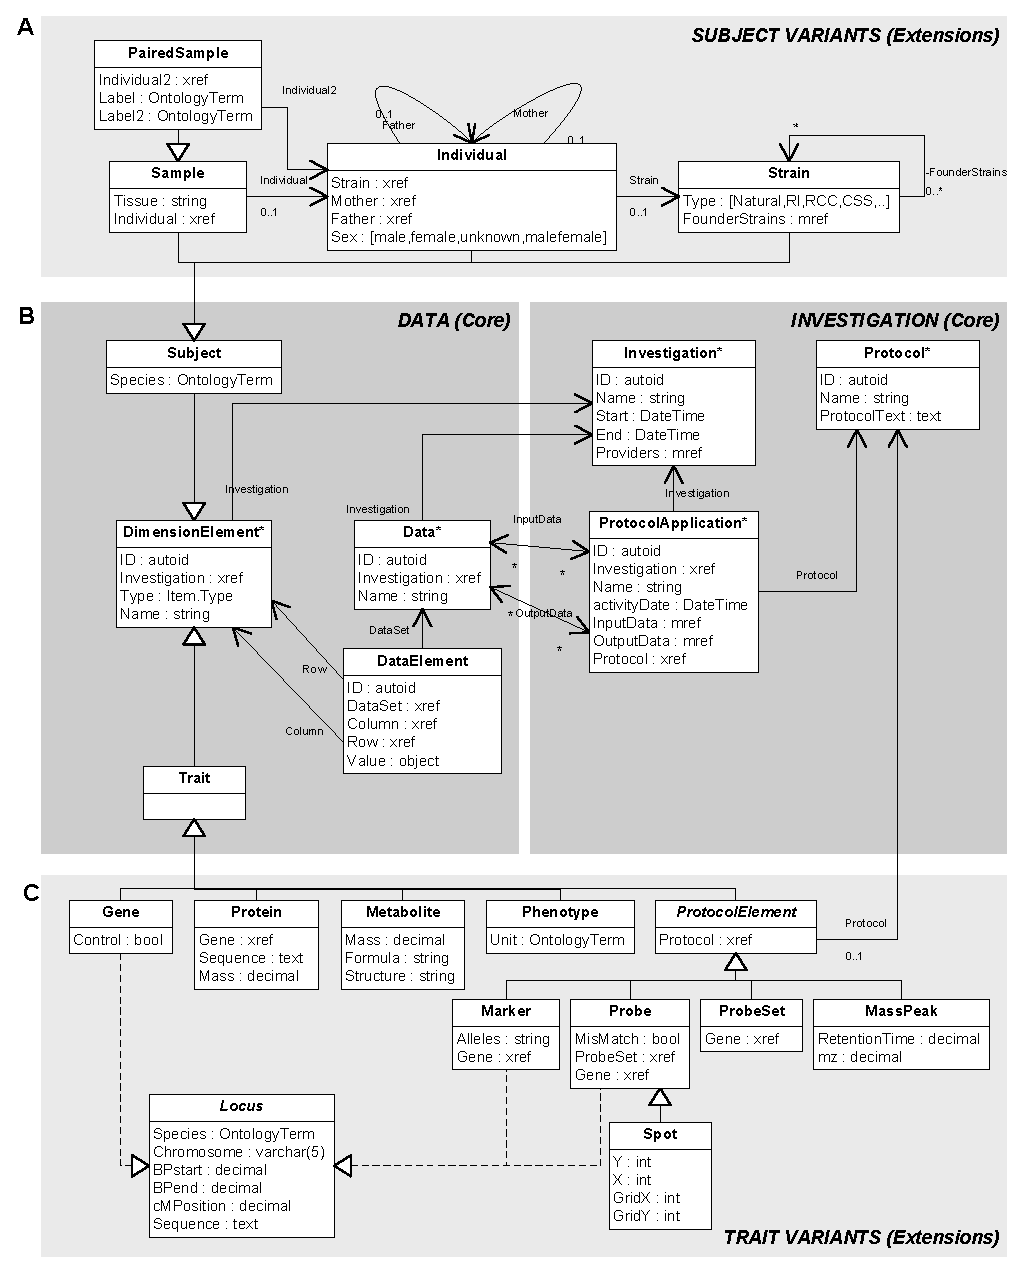
\includegraphics[width=0.81\textwidth]{eps/image_5_3.eps}
  \caption[XGAP.]
    {Experimental genotype and (molecular) phenotype data can be described using Subject, Trait, Data and DataElement; 
    the experimental procedures used can be described using Investigation, Protocol and ProtocolApplication (B). Specific 
    attributes and relationships can be added by extending core data types, e.g. Sample and Gene (A,C). The model is 
    described in UML: Arrows denote relationships (Data has a field Investigation that refers to Investigation ID); 
    Triangled lines denote inheritance (Metabolite inherits all properties ID, Name, Type from Trait, next to mass, 
    formula and structure); Triangled dotted lines denote use of interface (Spot 'implements' properties of Locus); 
    relationships are shown both as arrows and as properties ('xref' for one-to-many , 'mref' for many-to-many 
    relationships). Asterisk* marks FuGE derived types.}
    \label{fig:XGAP}
\end{figure}

We describe these biological components using FuGE data types and XGAP extensions thereof. 
Investigation binds all details of an investigation. Each investigation may apply a series 
of bio molecular \cite{Brown:2005} and computational \cite{Carey:2007,Alberts:2008,Fu:2007,Bhave:2007} 
Protocols. The applications of such Protocols are termed ProtocolApplications, which in the case 
of computational Protocols may require 
input Data and will deliver output Data.These data have the form of matrices, the DataElements 
of which have a row and a column index. Each row and column refers to a DimensionElement, 
being a particular Subject or a particular Trait, Table 2 illustrates the usage of these core 
data types. Figure \ref{fig:XGAP}a and \ref{fig:XGAP}c shows how the XGAP model can be extended to accommodate details on 
particular types of subjects and traits in a uniform way. A Trait can be a classical phenotype 
(for example, flowering - the flowering time is stored in the DataElement) or a bio molecular 
phenotype (for example, Gene X it's transcript abundance is stored in the DataElement). A 
Trait can also be a genotype (for example, Marker Y is a genomic feature observation that is 
stored in the DataElement). Genomic traits such as Gene, Marker and Probe all need additional 
information about their genome Locus to be provided. Similarly, a Subject can be a single 
Sample (for example, a labeled biomaterial as put on a microarray) and such a sample may 
originate from one particular Individual. It may also be a PairedSample when biomaterials come 
from two individuals - for example, if biomaterial has been pooled as in two-color microarrays. 
An individual belongs to a particular Strain. When new experiments are added new variants of 
Trait and Subject can be added in a similar way. Table 3 illustrates the generic usage of 
these extended data types.

Several standard data types were also inherited from FuGE to enable researchers to provide 
'Minimum Information' for QTLs and Association Studies such as defined in the MIQAS checklist 
 - a member of the Minimum Information for Biological and Biomedical Investigations (MIBBI) 
guideline effort \cite{Taylor:2008}

\subsection{Conclusions and Discussion}
In this paper we report a minimal and extensible data infrastructure for the management and 
exchange of genotype-to-phenotype experiments, including an object model for genotype and 
phenotype data (XGAP-OM), a simple file format to exchange data using this model (XGAP-TAB) 
and easy-to-customize database software (XGAP-DB) that will help groups to directly use and 
adapt XGAP as a platform for their particular experimental data and analysis protocols. We 
successfully evaluated the XGAP model and software in a broad range of experiments: array 
data (gene expression, including tiling arrays for detection of alternative splicing, 
ChIP-on-chip for methylation, and genotyping arrays for SNP detection); proteomics and 
metabolomics data (liquid chromatography time of flight mass spectrometry (LC-QTOF MS), NMR); 
classical phenotype assays \cite{Heap:2009, Bystrykh:2005, Li:2006, Keurentjes:2006, Stranger:2007, Bailey:2008, Beamer:1999}; 
other assays for detection of genetic markers; and annotation information for panel, gene, 
sample and clone. Non-technical partners successfully evaluated the practical utility by 
independently formatting and loading parts of their consortium data: EU-CASIMIR (for mouse), EU-GEN2PHEN (for human), 
EU-PANACEA (for \emph{C. elegans}) and IOP-Brassica (for plants). A public subset of these data sets 
is available for download at \url{http://www.xgap.org}. When needed we could quickly add customizations to the 
model, building on the general schema, and then use MOLGENIS to generate a new version of the 
software at the push of a button, for example, to support NMR methods as an extended type of 
Trait \cite{Fu:2009}. Furthermore we successfully integrated processing tools, such as a two-way 
communication with R/QTL \cite{Broman:2003, Arends:2010} enabling QTL mapping on XGAP 
stored genotypes and phenotypes with QTL results stored back into XGAP.

Based on these experiences, we expect use of XGAP to help the community of genome-to-phenome 
researchers to share data and tools, notwithstanding large variations in their research aims. 
The XGAP data format can be used to represent and exchange all raw, intermediate and result 
data associated with an investigation, and an XGAP database, for instance, can be used as a 
platform to share both data and computational protocols (for example, written in the R 
statistical language) associated with a research publication in an open format. We envision 
a directory service to which XGAP users can publish metadata on their investigations either 
manually or automatically by configuring this option in the XGAP administration user interface. 
This directory service can then be used as an entry point for federated querying between the 
community of XGAPs to share data and tools. Groups that already have an infrastructure can 
assimilate XGAP to ease evolution of their existing software.

Next to their existing user tools, they can 'rewire' algorithms and visual tools to also use 
the MOLGENIS APIs as data backend. Thus, researchers still have the same features as before, 
plus the features provided by the generated infrastructure (for example, data management GUIs, 
R/API) and connected tools (for example, R packages developed elsewhere). Moreover, much 
less software code needs to be maintained by hand when replacing hand-written parts by 
MOLGENIS-generated parts,  allowing software engineers to add new features for researchers 
much more rapidly. We invite the broader community to join our efforts at the public XGAP.org 
wiki, mailing list and source code versioning system to evolve and share the best XGAP 
customizations and GUI/API 'plug-in' enhancements, to support the growing range of profiling 
technologies, create data pipelines between repositories, and to push developments in the 
directions that will most benefit research

\section{High throughput data analysis (xQTL workbench)}
xQTL workbench is a scalable web platform for the mapping of quantitative trait loci (QTLs) 
at multiple levels: for example gene expression (eQTL), protein abundance (pQTL), metabolite 
abundance (mQTL) and phenotype (phQTL) data. Popular QTL mapping methods for model organism 
and human populations are accessible via the web user interface. Large calculations scale 
easily on to multi-core computers, clusters and Cloud. All data involved can be uploaded 
and queried online: markers, genotypes, microarrays, NGS, LC-MS, GC-MS, NMR, etc. When new 
data types come available, xQTL workbench is quickly customized using the MOLGENIS software 
generator.

Modern high throughput technologies generate large amounts of genomic, transcriptomic, proteomic, 
and metabolomic data. However, existing open source web-based tools for QTL analysis, such as 
webQTL \cite{Wang:2003} and QTLNetwork \cite{Yang:2008}, are not easily extendable to different 
settings and computationally scalable for whole genome analyses. \xqtlwb makes it easy to analyse 
large and complex datasets using state-of-the-art QTL mapping tools and to apply these methods 
to millions of phenotypes using paralellized 'Big Data' solutions\cite{Trelles:2011}. 
\xqtlwb also supports storing of raw, intermediate and final result data, and analysis protocols 
and history for reproducibility and data provenance. Use of MOLGENIS\cite{Swertz:2010b} 
helps to customize the software. All is conveniently accessible via standard Internet browsers on 
Windows, Linux or Mac (and using Java, R for the server).

\subsection{Features}
\xqtlwb provides visualization of QTL profiles, single and multiple QTL mapping methods, easy addition 
of new QTL analyses, scalable data management and analysis tracking.

\begin{figure}[h!]
  \centering
  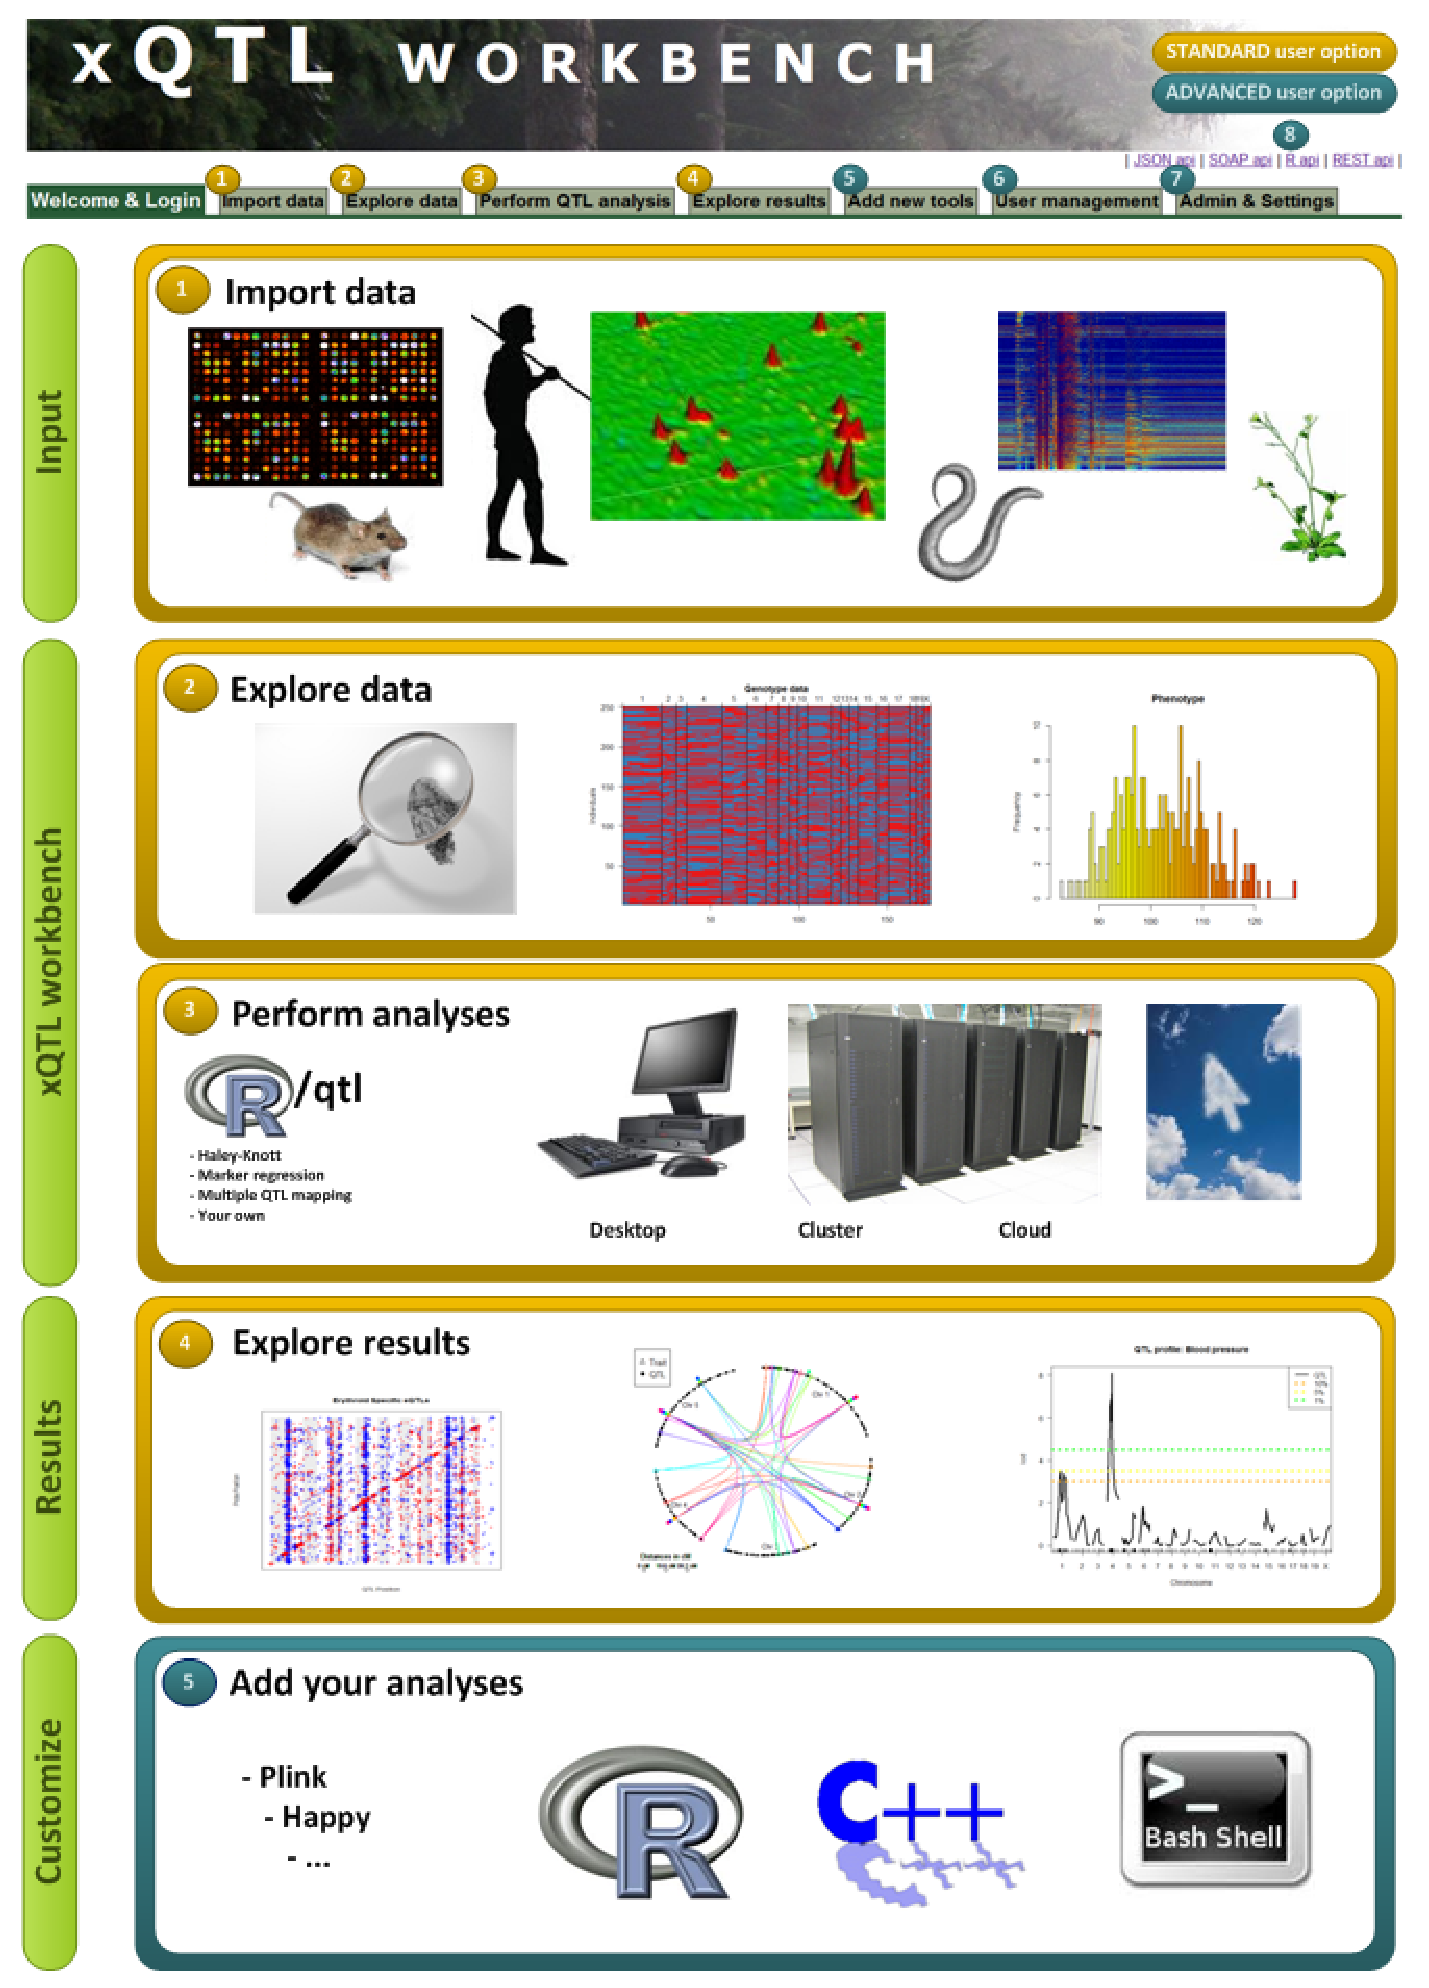
\includegraphics[width=0.75\textwidth]{eps/image_5_4.eps}
  \caption[xQTL workbench.]{Screenshot of xQTL workbench with all features enabled, (1) Import phenotype, genotype 
          and genetic map data, examples are given per import type; (2) Search through the whole database, explore 
          and browse your data using MOLGENIS generated web-interfaces; (3) Run R/qtl QTL mapping, the general 
          plugin allows users to perform not only QTL mapping but also other analyses; (4) Use default (or custom) 
          plugins to explore results (e.g. Heatmaps, QTL profiles); (5) Add new tools to the workbench (for 
          Bioinformaticians); (6) User management and access control of the system (Only for admins); (7) Expert 
          settings can be altered in the admin tab (Only for admins); (8) Connect/share data using generated API's 
          to R statistics, REST/JSON, SOAP.}
          \label{fig:xQTLworkbench}
\end{figure}

\begin{enumerate}\itemsep1pt
\item \emph{Explore QTL profiles} - Through the web-interface, users can explore mapped QTLs, and 
underlying information by viewing QTL plots in an interactive scrollable and zoomable window. 
\xqtlwb has support for other common image formats, such as PNG, JPG, SVG and embedded postscript; 
useful for publishing scientific results online, and on paper. From the output, main database identifiers, 
such as gene, protein and/or metabolite identifiers are automatically linked-out to matching external 
web pages of public database such as NCBI, KEGG, and Wormbase.
\item \emph{Single and multiple QTL mapping} - \xqtlwb wraps R/qtl \cite{Broman:2003, Arends:2010} in a 
web-based analysis framework offering all important QTL mapping routines, such as the EM algorithm, 
imputation, Haley-Knott regression, the extended Haley-Knott method, marker regression, and Multiple 
QTL mapping. In addition, \xqtlwb includes R/qtlbim, a library which provides a Bayesian model 
selection approach for mapping multiple interacting QTL \cite{Yandell:2007} and Plink, a library for 
association QTL mapping on Single Nucleotide Polymorphisms (SNP) in natural populations \cite{Purcell:2007}.
\item \emph{Add new analysis tools} - \xqtlwb supports flexible adding of more QTL analysis software: 
any R-based, or command-line tool, can be plugged in. All analysis results are uploaded, stored and 
tracked, in the \xqtlwb database through an R-API. When new tools are added, they can build on the 
high-level multi-core computer, cluster and Cloud management functions, based on TORQUE/OpenPBS and 
BioNode \cite{Prins:2012}. \xqtlwb can be made part of a larger analysis pipeline using interfaces to R, 
Excel, REST and SOAP web services and Galaxy \cite{Goecks:2010}.
\item \emph{Track and trace} - When a new analysis protocol or R script is defined, this protocol 
can easily be applied to new data. Also, \xqtlwb keeps track of history. Re-use of analysis protocols 
can be done in an automated fashion. Previous analyses can be rerun without resetting parameters. 
\xqtlwb provides an online overview of past analyses e.g. which analyses were performed, by who, when 
and display settings applied.
\item \emph{Scalable data management} - \xqtlwb has a consistency checking database based on XGAP 
specification \cite{Swertz:2010a}, user interfaces to manage and query genotype and phenotype data 
sets, and support for various database back-ends including HSQL (standalone) and MySQL. Phenotype, 
genotype and genetic map data can be imported as text (TXT), comma separated (CSV), and Excel files. 
\xqtlwb handles and stores large data in a new and efficient binary edition of the XGAP format, named 
XGAPbin (extension .xbin), documented online. Such binary formats are essential when handling, storing 
and transporting multi-Gigabyte datasets.
\item \emph{Customize to research} - Additional modules for new data modalities can be added using 
MOLGENIS software generator \cite{Swertz:2010b}. The 'look and feel' of \xqtlwb is adaptable to 
institute or consortium style by changing a simple template which is described in the \xqtlwb 
documentation enabling seamless integration into an existing web-site or intranet site, such as 
recently for EU-PANACEA model organism project and LifeLines biobank.
\end{enumerate}

\subsection{Implementation}
We built \xqtlwb on top of MOLGENIS \cite{Swertz:2004}, a Java based software to generate tailored 
research infrastructure on-demand \cite{Swertz:2007}. From a single 'blueprint' describing the whole 
system, MOLGENIS auto-generates a full application including user interface, database infrastructure, 
application programming interfaces in R, REST and SOAP (APIs). MOLGENIS' flexibility and robustness 
is proven by the wide range of research projects, e.g. the Nordic GWAS Control database \cite{Leu:2010}, 
EB mutation database \cite{Akker:2011}, the Animal observation database \cite{Swertz:2010b}.

For data storage, the eXtensible Genotype and Phenotype (XGAP) data model was adopted \cite{Swertz:2010a} 
and extended for big data. To support the increased demand for computational resources for included 
mapping routines we added high-level cluster and cloud management functions for computation. The 
scalable QTL mapping routines of \xqtlwb are written in R and C. The choice of R ties in with the 
general practice of using R for QTL mapping. The user interface includes direct access to the R 
interpreter. Both \xqtlwb and MOLGENIS are open source software, and source code is transparently
stored and tracked in online source control repositories.

\subsection{Conclusions and Discussion}
\xqtlwb provides a total-solution for web-based analysis: Major QTL mapping routines are integrated 
for use by experienced and inexperienced users. Researchers can upload raw data, run analyses, explore 
mapped QTL and underlying information, and link-out to important databases. New algorithms can be 
flexibly added, immediately available to all users. Large analyses can be easily executed on a cluster, 
or in the Cloud. Future work include visualizations and search options to explore the results. We also 
had an EU-SYSGENET workshop that envisioned further integration of xQTL with analysis tools like HAPPY, 
databases like GeneNetwork, and the workflow manager TIQS \cite{Durrant:2012}.

\section{A worm database (WormQTL)}
WormQTL is one of the application developed using the xQTL workbench system. It is a public web portal 
for the management of all these new data and integrated development of suitable analysis tools. The 
web server provides a rich set of analysis tools available to use directly, based on R/qtl 
\cite{Broman:2003, Arends:2010}. Users can upload and share new R scripts as 'plugin' for colleagues 
in the community to use directly. New data can be uploaded and downloaded using XGAP-extensible 
text format for genotype and phenotypes\cite{Swertz:2010a}. All data and tools can be accessed 
via web user interfaces and programming interfaces to R, REST, and SOAP web services. Large 
consortia as well as individual researchers, can have a private area that is under embargo for 
publication. All software is free for download as MOLGENIS 'app' \cite{Swertz:2010b}. WormQTL is 
freely accessible without registration and is hosted on a large computational cluster enabling 
high throughput analyses to all at:\\
\url{http://www.wormqtl.org/}.

\subsection{Background}

Over the past 30 years, the metazoan \emph{Caenorhabditis elegans} has become a premier animal model for 
determining the genetic basis of quantitative traits \cite{Gaertner:2010, Kammenga:2008}. The 
extensive knowledge of molecular, cellular and neural bases of complex phenotypes makes 
\emph{C. elegans} an ideal system for the next endeavor: determining the role of natural genetic 
variation on system variation. These efforts have resulted in an accumulation of a valuable amount 
of phenotypic, high-throughput molecular and genotypic data across different developmental worm 
stages and environments in hundreds of strains \cite{Palopoli:2008, Kammenga:2007, Rockman:2010, 
McGrath:2009, Reddy:2009, Doroszuk:2009, Li:2010, Gutteling:2007, Vinuela:2010}. In addition, a similar wealth has been 
produced on hundreds of different \emph{C. elegans} wild isolates and other species \cite{Andersen:2012}. 
For example, \emph{C. briggsae} is an emerging model organism that allows evolutionary comparisons 
with \emph{C. elegans} and quantitative genetic exploration of its own unique biological 
attributes \cite{Ross:2011}.

This rapid increase in valuable data calls for an easily accessible database allowing for 
comparative analysis and meta-analysis within and across Caenorhabditis species \cite{Swertz:2007}. To 
facilitate this, we designed a public database repository for the worm community, WormQTL 
(\url{http://www.wormqtl.org/}). Driven by the PANACEA project of the systems biology program of 
the EU, its design was tuned to the needs of \emph{C. elegans} researchers via an intensive 
series of interactive design and user evaluation sessions on a mission to integrate all 
available data within the project.

As a result, data that were scattered across different platforms and databases can now be 
stored, downloaded, analysed and visualized in an easily and comprehensive way in WormQTL. 
On top, the database provides a set of user interfaced analysis tools to search the database 
and explore genotype-phenotype mapping based on R/qtl \cite{Broman:2003, Arends:2010}. New 
data can be uploaded and downloaded using the extensible plain text format for genotype and 
phenotypes, XGAP \cite{Swertz:2010a}. There is no limit to the type of data (from gene 
expression to protein, metabolite or cellular data) that can be accommodated because of its 
extensible design. All data and tools can be accessed via a public web user interface and 
programming interfaces to R and REST web services, which were built using the MOLGENIS 
biosoftware toolkit \cite{Swertz:2010b}. Moreover, users can upload and share more R 
scripts as 'plugin' for the colleagues in the community to use directly and run those on a 
computer cluster using software modules from xQTL workbench \cite{Arends:2012, Snoek:2012}; this requires 
login to prevent abuse. All software can be downloaded for free to be used, for example as 
local mirror of the database, and/or to host new studies.

All the software was built as open source, reusing and building on existing open source components 
as much as possible. WormQTL is freely accessible without registration and is hosted on a large 
computational cluster enabling high-throughput analyses. Below we detail the results and future plans.

\subsection{Results}
WormQTL is an online database platform for expression quantitative trait loci (eQTL) exploration 
to service the worm community and already provides many publicly available data sets \cite{Rockman:2010, 
Doroszuk:2009, Li:2006, Li:2010, Gutteling:2007, Vinuela:2010, Elvin:2011, Vinuela:2012}. New data 
sets can be uploaded using the XGAP plain file data format. Suitable help pages are provided. 
Currently, 38 public data sets have been loaded, of which the bulk is xQTL data on 500 strains 
(introgression lines, recombinant inbred lines (RILs), recombinant inbred advanced intercross lines 
and natural isolates), 55,000 transcripts, 1594 samples and 1579 markers (Table 1). With this 
combination of classical phenotypes, molecular profiles and genetics data sets, WormQTL contains 
all the 'genetical genomics' experiments published to our current knowledge (except for some tiling 
data). Using WormQTL, researchers can explore many xQTLs across the various studies in different 
conditions and ages and compare classical QTLs with xQTLs. The main interfaces are 'Find QTLs', 
'Genome browser' and 'Browse data'.

\begin{enumerate}\itemsep1pt
\item \emph{Find QTLs} - QTL is genomic regions associated with phenotypic variation and can be 
used to study the genetic architecture of traits and to detect potential phenotypic regulators. 
Recently, the number of QTLs and especially eQTL studies in \emph{C. elegans} has increased greatly. 
These eQTL studies consist of large data sets that, before WormQTL, were very difficult to access 
and perform a combined meta-analysis. Therefore, we provide easy access to most of the eQTL studies 
published, by search, browse and plot functions (Figure \ref{fig:xQTLworkbench}). We support relatively simple questions like 
'does my gene have an xQTL?' to more advanced ones like 'how do these genes fit into an xQTL network?'. 
All the matching genes, markers and traits found in the data sets are returned including links to 
WormBase and literature. Furthermore, WormQTL is the first portal for any species that allows comparison 
of eQTLs over multiple experiments and environments, giving insight in the plastic nature of genetic 
regulation.
\item \emph{Genome browser} - To find the genes that have a QTL on your favorite position, click 
'Genome browser'. Here, you can select from all the different releases of the University of California, 
Santa Cruz genome releases. You can add tracks from the designated experiments of interest. Then 
navigate to your favorite location (tip: use open in new window) and collect significant probe 
identifiers from that region.
\item \emph{Browse data} - Complete data sets and accompanying gene, sample and trait identifier 
lists can be browsed via the 'browse data' user interface. External identifiers anywhere in the 
data are automatically recognized and enhanced as linkouts to background information, such as links 
to Wormbase, NCBI, KEGG or Ensembl. All the annotation lists and data matrices can be browsed and 
searched in a tabular form and can be downloaded as plain text or Excel files. Readers can also 
download data sets or submit new data sets using the XGAP data format following examples described 
in the WormQTL help section. Also all data can be accessed programmatically from with R (as whole 
matrix or per row) or using REST web services, including filtering of the annotations (genes, probes, 
markers and phenotypes) and services to 'slice' individual lines out of the complete data sets to 
speed up download and (parallel) analyses. Alternatively, readers can request a login to upload 
data and new analysis scripts directly.
\end{enumerate}

\subsection{Conclusions and Discussion}
\subsubsection{Implementation}
All the software was implemented using the open source Molecular Genetics Information Systems 
MOLGENIS toolkit \cite{Swertz:2010a}, and in particular one previously existing MOLGENIS application, the 
extensible xQTL workbench \cite{Arends:2012} and the R/qtl QTL mapping and visualization package for the R 
language \cite{Broman:2003, Arends:2010}. The MOLGENIS toolkit is a Java-based software to generate tailored research 
infrastructure on demand \cite{Swertz:2007}. From a single 'blueprint' describing all biological data 
structures and user interfaces of the whole system, MOLGENIS auto generates a full application 
including user interface, database infrastructure and application programming interfaces 
(APIs) in R, REST and SOAP.

At the push of a button, MOLGENIS 'generators' automatically translates these models into a 
database, standard user interfaces for data queries and updates, upload/download tools for 
tab-delimited data and scriptable interfaces for programmers to users from within R and via 
web services. This greatly speeded up the initial software development and also enables rapid 
extension when, for example, new data types arrive. On top of this foundation, we build the 
WormQTL specific user interactions such as the 'Find QTLs' and the 'Genome browser' using 
MOLGENIS 'plug-in' mechanism and the visualizations and plots using the R interface. xQTL 
workbench is a scalable web platform for the mapping of QTLs at multiple levels: for example, 
gene expression (xQTL), protein abundance (pQTL), metabolite abundance (mQTL) and phenotype 
(phQTL) data. The xQTL workbench provided a set of previously developed user interfaces to 
run R/qtl mapping methods directly from within the WormQTL user interface, the ability to 
add new analysis procedures in R, data management and data format conversions, all greatly 
speeding up the generation of new xQTL profiles.

All the data sets were downloaded from their original sources and then formatted using the 
XGAP data format. XGAP is a simple text file format that uses a directory of tab-delimited 
files or one Excel file with multiple sheets to load lists of annotations and data matrices. 
The annotations list all the background information needed to run and interpret the analysis 
including, for example, genome position information, such as markers, genes, probes and 
strains. The data matrices describe all the raw, intermediate and result data, such as gene 
expression, genotypes and QTL P-values, with the row names and column names cross linking to 
the annotations. For example, gene expression is a matrix of 'gene' X 'sample'. Subsequently 
these data sets were loaded using the MOLGENIS/xQTL data import wizards, which check the 
files for correctness and give informative feedback if the data are not yet in a format that 
WormQTL can understand \cite{Swertz:2010a}. All the annotations are stored in tables in the database; the 
large data matrices are stored in a optimized binary format to speed up analyses and queries. 
This format is documented in the WormQTL manual to ease the submission of new data sets from 
the community. Finally, all the QTL profiles were recalculated according to the specification 
of the original, or slightly modified when needed, such as to include a previously missing 
wrongly labelled sample correction. In this process, we greatly benefitted from the integration 
with xQTL workbench, which enabled us to re-run all these analyses on the computer cluster 
and add new R analysis procedures when needed, simply from the user interface.

All software is available as open source on \url{http://github.com/molgenis/} for others to reuse 
locally, and related technical documentation is available from:\\ \url{http://www.xqtl.org/}, 
\url{http://www.rqtl.org/} and \url{http://www.molgenis.org/}.

\subsubsection{Future plans}
The current version of WormQTL (June 2012) is a comprehensive, versatile and flexible package. 
Follow-up plans of more extended versions with new tools and data depend on the demand by the 
users of WormQTL. We envisage that in the future, three types of new tools will be developed: 
(i) visualization tools, (ii) QTL mapping tools and (iii) candidate gene selection tools. Improved 
visualization tools might include plotting a phenotype against the marker at a certain position; 
so the two groups become visible at a QTL position. Also plots can be made showing transgression 
and heritability per microarray probe or gene or histograms of the phenotypic values (and include 
the parental values if available). Advanced QTL mapping tools might include multi-environment
/age mapping or genotype-by-environment analyses, developed in collaboration with the R/qtl team 
to enable automatic links to this software. The candidate gene selection tools would benefit from 
the most recent stable release of Wormbase \cite{Yook:2012}, the most widely used platform for worm biology. 
But also other sources of information like MODENCODE \cite{Gerstein:2010} or Wormnet 
\cite{Lee:2008} are likely to be connected with WormQTL. A candidate gene selection tool might be 
implemented in a next version 
of WormQTL as it is less easy to implement and often needs information beyond WormQTL. One can 
think of (i) which SNPs/genes/polymorphic genes/transcription factor binding sites and so forth 
are underlying a eQTL; (ii) which gene, underlying my xQTL, is linked to most of the genes 
having an xQTL; (iii) which genes are polymorphic and (iv) which other genotypes show a difference 
in expression and do they share polymorphisms with the parental strains of the RIL population 
that the xQTL was mapped in. Moreover, WormQTL can be easily expanded to other Caenorhabditis 
species \cite{Ross:2011}.

We believe that WormQTL, which will be continuously curated by the members of this international 
consortium, is a very attractive database for the growing community of quantitative genetics in 
worms researchers. We are committed to maintain data and software for the years to come and invite 
the community to add and share new data and ideas.

\subsection{Update 2013: wormQTL-HD}
Interactions between proteins are highly conserved across species. As a result, the molecular basis 
of multiple diseases affecting humans can be studied in model organisms that offer many alternative 
experimental opportunities. One such organism - \emph{Caenorhabditis elegans} - has been used to produce much 
molecular quantitative genetics and systems biology data over the past decade. We present WormQTLHD 
(Human Disease), a database that quantitatively and systematically links expression Quantitative 
Trait Loci (eQTL) findings in \emph{C. elegans} to gene-disease associations in man. WormQTLHD, available 
online at \url{http://www.wormqtl-hd.org/}, is a user-friendly set of tools to reveal functionally coherent
, evolutionary conserved gene networks. These can be used to predict novel gene-to-gene associations 
and the functions of genes underlying the disease of interest. We created a new database that links 
\emph{C. elegans} eQTL data sets to human diseases (34 337 gene-disease associations from OMIM, DGA, GWAS 
Central and NHGRI GWAS Catalogue) based on overlapping sets of orthologous genes associated to 
phenotypes in these two species. We utilized QTL results, high-throughput molecular phenotypes, 
classical phenotypes and genotype data covering different developmental stages and environments from 
WormQTL database. All software is available as open source, built on MOLGENIS and xQTL workbench. 


